\subsection{Турнирная селекция}\label{SetOfOperatorsAlgorithms:TournamentSelection}

Идентификатор: \textbf{TournamentSelection}.

Из популяции с равной вероятностью выбираются индивиды в количестве $ T $ (размер турнира), где $ 2\leq T\leq PopulationSize $ ($ PopulationSize $ --- размер популяции). При этом каждый индивид может попасть в группу (турнир) только один раз (турнирная селекция без возвращения). Из данной группы выбирается индивид с наибольшей пригодностью.

Значит, турнирная селекция определяется формулой:
\begin{align}
\label{SetOfOperatorsAlgorithms:eq:TournamentSelection}
Selection\left( Population, Fitness, DataOfSel\right) = \arg{\max_{\bar{x}\in H} {f_{fit}\left( \bar{x}\right) }}, \text{где }\\
H=\left\lbrace h^i | h_i=Random \left( Population/\left( \left\lbrace h^1\right\rbrace \cup \left\lbrace h^2\right\rbrace \cup \ldots  \cup \left\lbrace h^{i-1}\right\rbrace\right) \right) \right\rbrace, i=\overline{1,T}\nonumber.
\end{align}

Турнирная селекция добавляет в $ DataOfSel $ дополнительный параметр –-- размер турнира $ T $. Обычно выбирают значение этого параметра равное $ T=2 $.

\textbf{Пример.} Массив возьмем тот же, что и в предыдущих примерах $ Fitness=\left\lbrace 0,5; 0,2; 0,1; 0,6; 0,2; 0,4\right\rbrace $. Размер турнира равен $ T=3 $. Пример работы оператора показан на рисунке:

\begin{figure} [h] 
  \center
  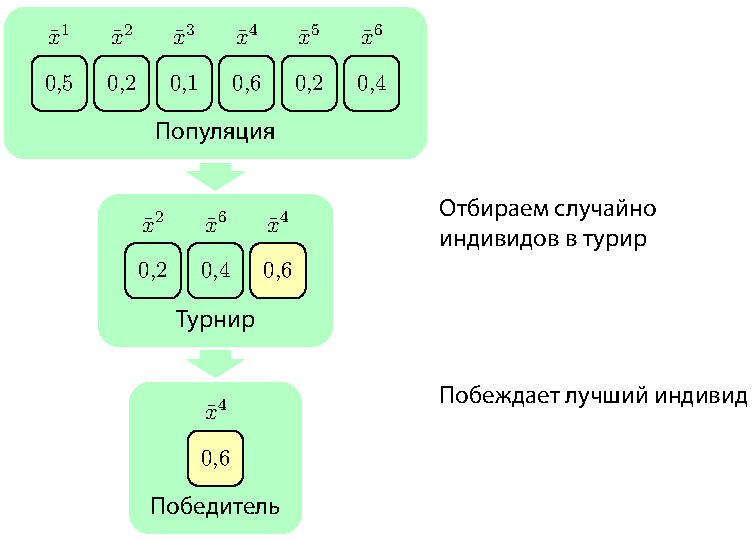
\includegraphics [scale=0.8] {TournamentSelection}
  \caption{Механизм работы турнирной селекции} 
  \label{SetOfOperatorsAlgorithms:img:TournamentSelection}  
\end{figure}

\begin{equation}
DataOfSel=\left( \begin{array}{c} TypeOfSel \\ T \end{array} \right).
\end{equation}

Нет ограничений на множество задач оптимизации, которые может решать алгоритм оптимизации с данной селекцией.

В библиотеке \textbf{HarrixMathLibrary} данная селекция реализуется через функцию \textbf{MHL\_TournamentSelection}:

\href{https://github.com/Harrix/HarrixMathLibrary}{https://github.com/Harrix/HarrixMathLibrary}